\documentclass{beamer}
\usepackage{pgfpages}
\usepackage{newtxtext,newtxmath} %time new roman
%\setbeameroption{show notes}
%\setbeameroption{show notes on second screen=right}
\usetheme{Warsaw}
\usepackage[french]{babel}

\usepackage{tikz}
\pgfdeclareimage[height=0.5cm]{le-logo}{}
%\setbeamertemplate{footline}[frame number]
%Set number slide 

\usepackage[backend=biber]{biblatex}
%\usepackage[backend=biber, style=chem-acs]{biblatex}
\addbibresource{presentation.bib} 
\bibliography{Skin Cancer Detection}
\setbeamertemplate{bibliography item}[triangle]

\usepackage{multirow}% row fusion
\usepackage{array} % column fusion
\usepackage{xfrac} % small fractions
\usepackage{adjustbox}
\usepackage{listings}
\usepackage{color}
\definecolor{gray}{rgb}{0.4,0.4,0.4}
\definecolor{darkblue}{rgb}{0.0,0.0,0.6}
\definecolor{cyan}{rgb}{0.0,0.6,0.6}
 \titlegraphic{\vspace{-1cm}
      
\includegraphics[width=2.5cm]{images/paris8_1}\hspace*{4.75cm}~%
      \hfill
      
\includegraphics[width=2.5cm]{images/tc_logo}
}
\setbeamertemplate{frametitle}{\nointerlineskip  
    \begin{beamercolorbox}[wd=\paperwidth,ht=2.75ex,dp=1.375ex]{frametitle}
        \hspace*{2ex}\insertframetitle \hfill {\small\insertframenumber/\inserttotalframenumber} \hspace*{1ex}%
    \end{beamercolorbox}}

\usecolortheme{wolverine}
\setbeameroption{hide notes} % Only slides


%%%%%%%%%%%%%%%%%%%%%%%%%%%
\title[Identification de la source d'une transaction] 
{Identification de store et de retailer à partir des données de paiement}
%\subtitle {ne compléter que si l'article possède un sous-titre}
\author[Komlan Dantodji] 
{Komlan Jean-Marie DANTODJI}

\institute[]
{
  Etudiant en M1 Big Data
  \and
  Université Paris 8}
\date{April 29, 2020}


\begin{document}
\begin{frame}
  \titlepage
\end{frame}

\begin{frame}{Plan}
  \tableofcontents
\end{frame}

\section{Introduction}
\subsection{Présentation de l'entreprise}
\begin{frame}{Transaction Connect}
\begin{itemize}
		\item Start Up de B2B2C aux retailers
		\item Editeur de solution numerique basé sur la donnée de paiement
\end{itemize}
\end{frame}

\subsection{Solution proposée}
\begin{frame}{Solution proposée}
\begin{itemize}
		\item Transaction Connect signe des contrats avec des foncières
		\item Fournit des services et outils de décision aux clients foncières (Dashboard, enrichissement des données)
		\item Transformation de la carte bancaire en carte de fidélité
		\item Notification et Validation des Cashbacks aux clients acheteurs
\end{itemize}
\end{frame}
\subsection{Les contrats avec les foncières}
\begin{frame}{Les contrats avec les foncières}
\begin{figure}[H]
    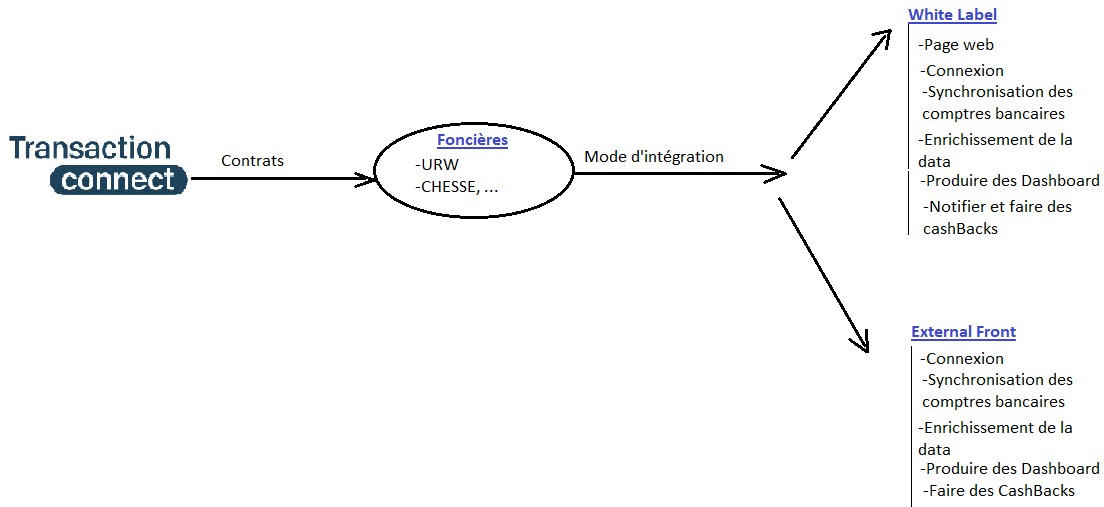
\includegraphics[width=11cm,height=4.8cm]{images/contrat.jpeg}
    \caption{[1] Les modes d'intégration}
    \label{fig:L1}
\end{figure}
\end{frame}

\subsection{Les moyens de connexion de transaction}
\begin{frame}{Les moyens de connexion de transaction}
\begin{figure}[H]
    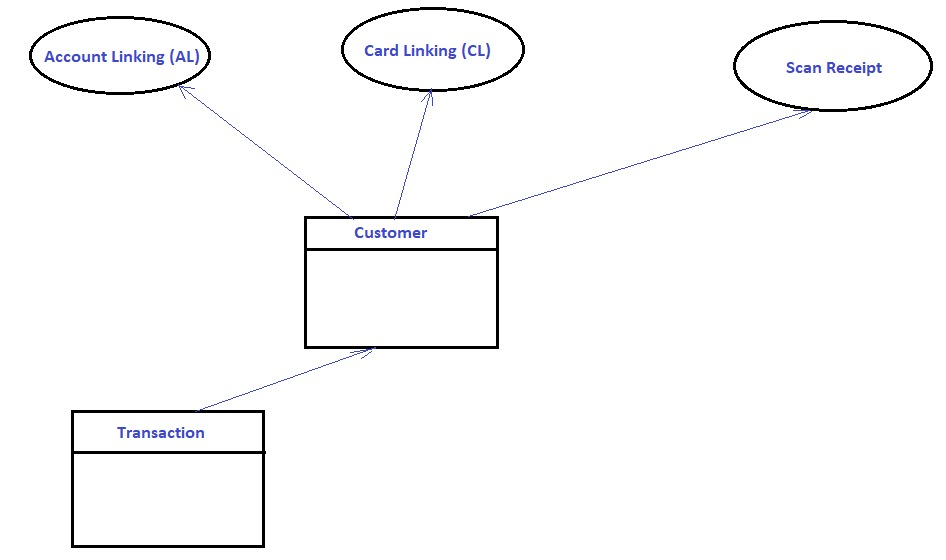
\includegraphics[width=11cm,height=4.8cm]{images/moyen_paiement.jpeg}
    \caption{[1] Les moyens de connexion de transaction}
    \label{fig:L1}
\end{figure}
\end{frame}

\section{Datasets}
\subsection{Source de donnée}
\begin{frame}{Source de données}
\begin{itemize}
		\item Les données proviennent des providers qui recupèrent les transactions auprès des Banques ("fidele", "Budget Insight")
		\item On dispose au total 119 tables dans la base de donnée
\end{itemize}
\begin{figure}[H]
    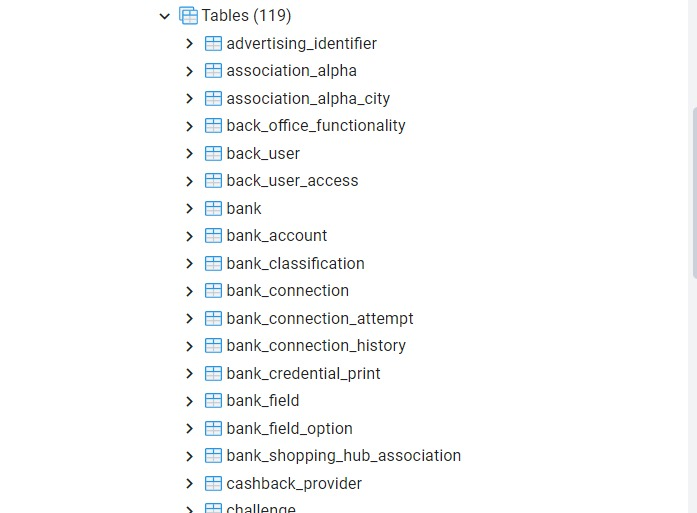
\includegraphics[width=11cm,height=4.8cm]{images/all_tables.jpeg}
    \caption{[1] Les moyens de connexion de transaction}
    \label{fig:L1}
\end{figure}
\end{frame}


\begin{frame}{Table de transaction (39 cols, 2361642 rows)}
\begin{figure}[H]
    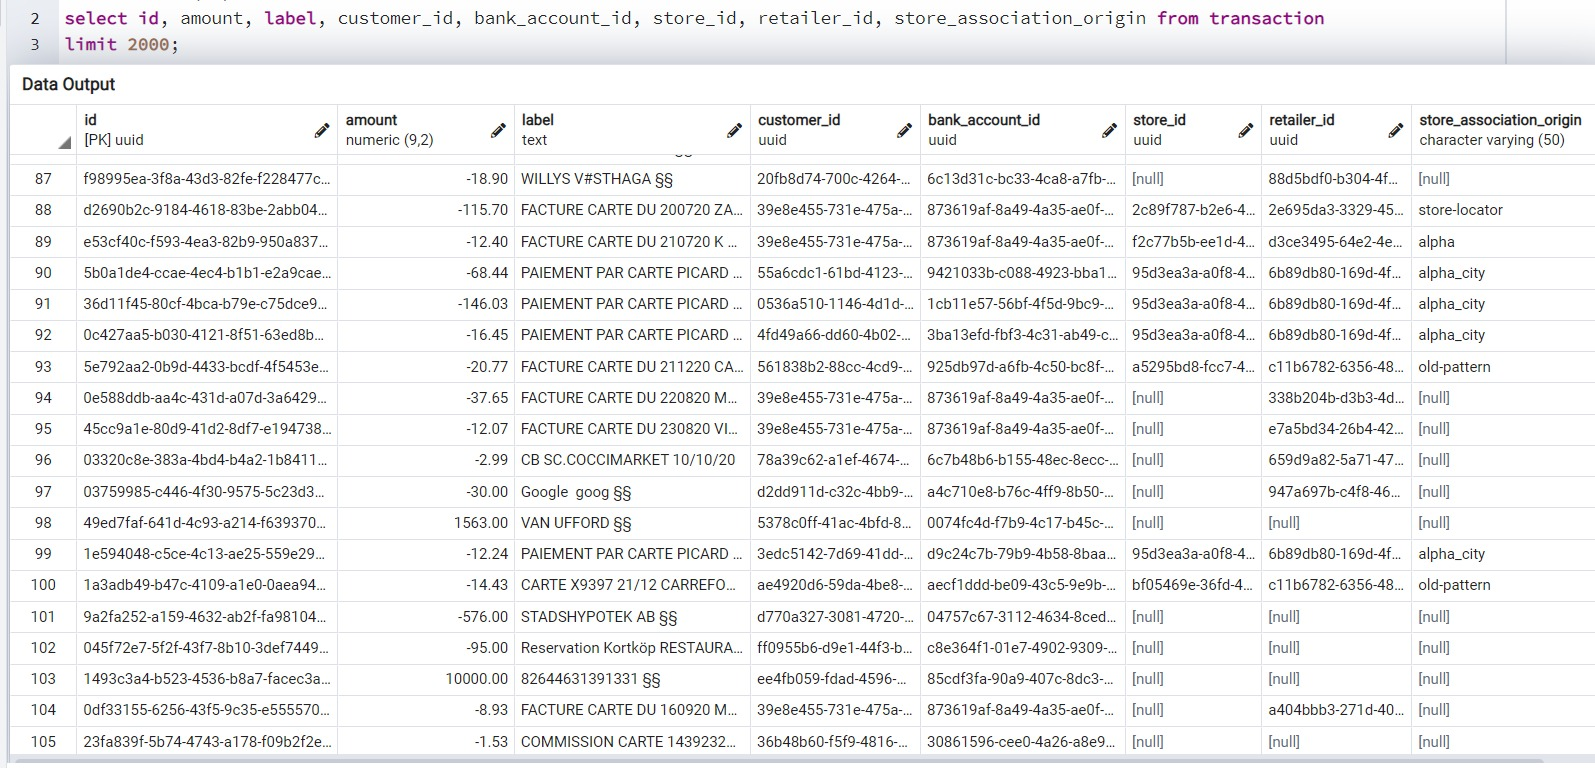
\includegraphics[width=11cm,height=5.2cm]{images/transaction.jpeg}
    \caption{[1] Les moyens de connexion de transaction}
    \label{fig:L1}
\end{figure}
\end{frame} 

\begin{frame}{Table des stores (33 cols, 125767 rows) }
\begin{figure}[H]
    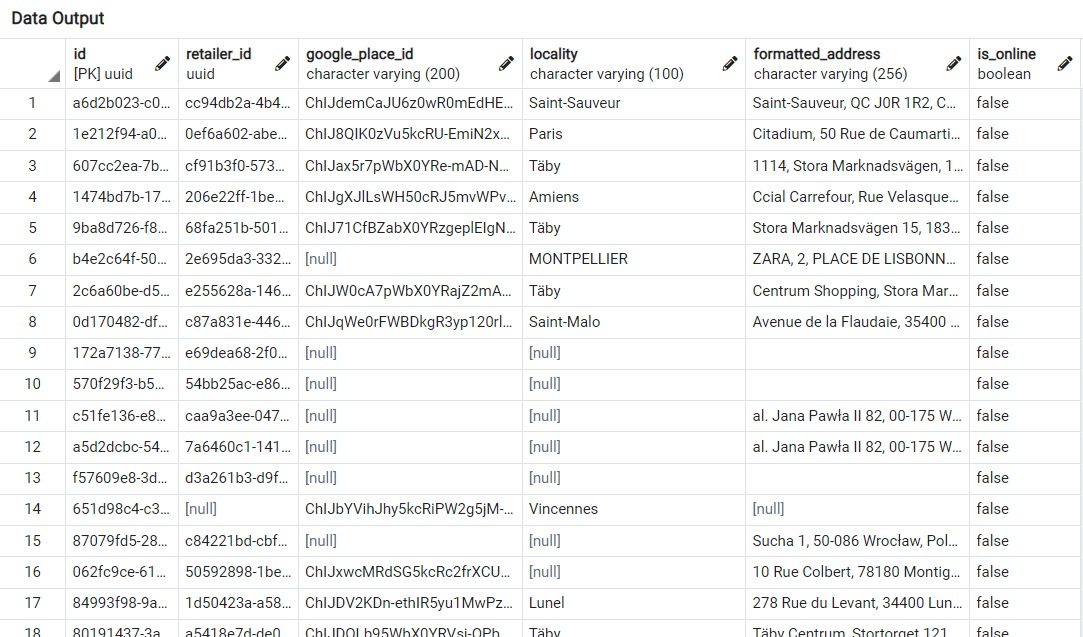
\includegraphics[width=11cm,height=5cm]{images/stores.jpeg}
    \caption{[1] Les moyens de connexion de transaction}
    \label{fig:L1}
\end{figure}
\end{frame} 

\section{Problématique}
\begin{frame}{Problématique}
\begin{itemize}
		\item Identifier dans quel store le client a effectué le paiement 
		\item En se basant sur le label contenu dans la transaction
		\item EX: "CB MONOPRIX 0295 02/03/21 10€" 
\end{itemize}
\end{frame} 

\section{Etat de l'art}
\begin{frame}{Etat de l'art}
\begin{itemize}
		\item API Google Place ID pour détecter une région à partir de la ville et un lieu connu
\end{itemize}
\end{frame} 

\section{Algorithmes utilisés}
\subsection{Algorithmes utilisés}
\begin{frame}{Algorithmes utilisés}
\begin{itemize}
		\item Store Locatore (connaissant le Retailer et la Ville)
		\item Scoring (basé sur la probabilité)
		\item Alpha / Alpha City (avec l'API Google MAP)
		\item Patterns Regrex 
		
\end{itemize}
\end{frame} 

\subsection{Algorithmes de Store Locator}
\begin{frame}{Algorithmes de Store Locator}
\begin{itemize}
		\item Initialiser toutes les villes, regions du pays dans un arbre
		\item Initialiser les Shoppings Hub (Les centres commerciaux de la region)
\end{itemize}
\begin{figure}[H]
    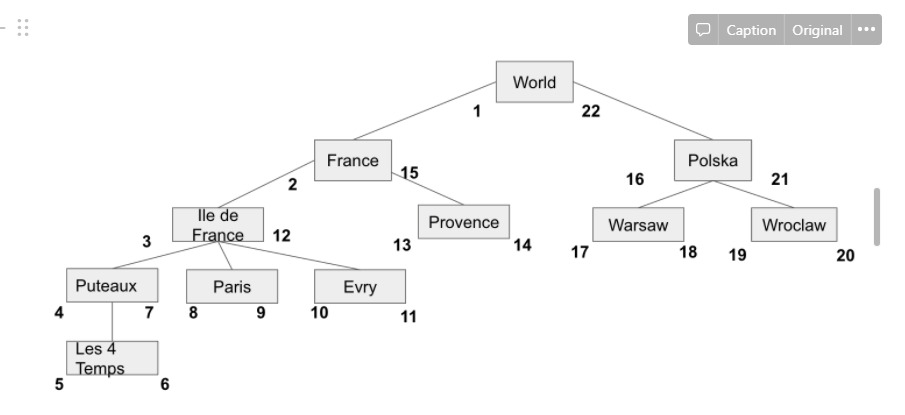
\includegraphics[width=11cm,height=4.3cm]{images/arbre.jpeg}
    \caption{[1] Arbre des zones géographiques}
    \label{fig:L1}
\end{figure}
\end{frame} 
\begin{frame}{Algorithmes de Store Locator}
\begin{itemize}
		\item Ajouter des patterns de détection des mots clés dans les labels (EX: marque, Numero de store, ville)
		\item Faire du monitoring pour modifier les patterns qui ne détectent pas de zone de transaction
\end{itemize}

\end{frame}





\section{Conclusion}
\begin{frame}{Conclusion}
\begin{itemize}
		\item Pour le moment je suis à létape de l'initialisation de store locatore pour la Grande Bretagne. 
\end{itemize}
\end{frame}


\begin{frame}
  \begin{block}{}
  \centering
  Merci pour votre attention...
  \end{block}
\end{frame}
\end{document}
